% begin module transformations-magnifications
\begin{frame}
\begin{columns}[c]
\column{.5\textwidth}
\ \only<handout:0| -2>{%
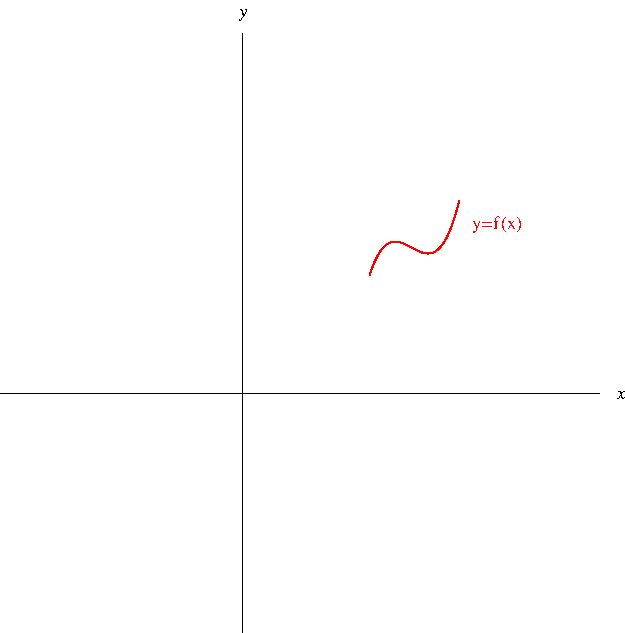
\includegraphics[height=5cm]{precalculus/pictures/01-03-maga.pdf}%
}%
\only<handout:0| 3>{%
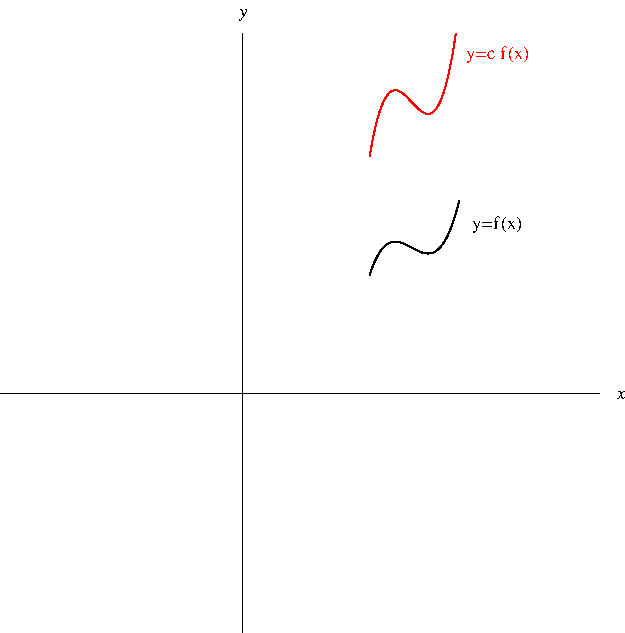
\includegraphics[height=5cm]{precalculus/pictures/01-03-magb.pdf}%
}%
\only<handout:0| 4>{%
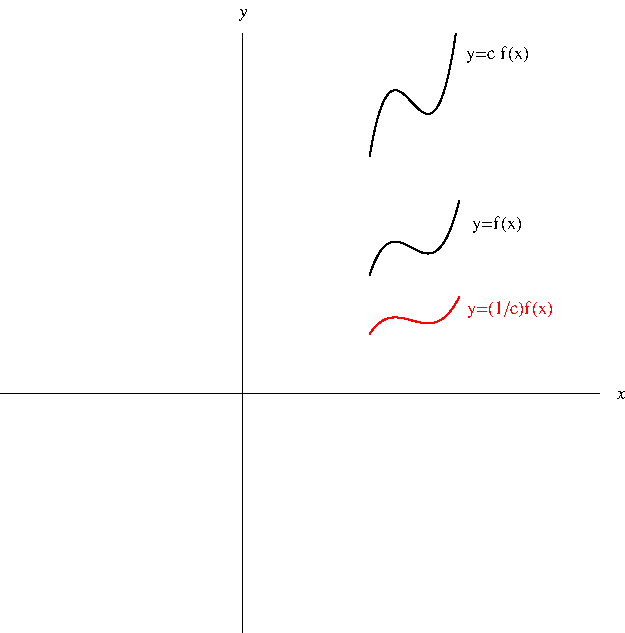
\includegraphics[height=5cm]{precalculus/pictures/01-03-magc.pdf}%
}%
\only<handout:0| 5>{%
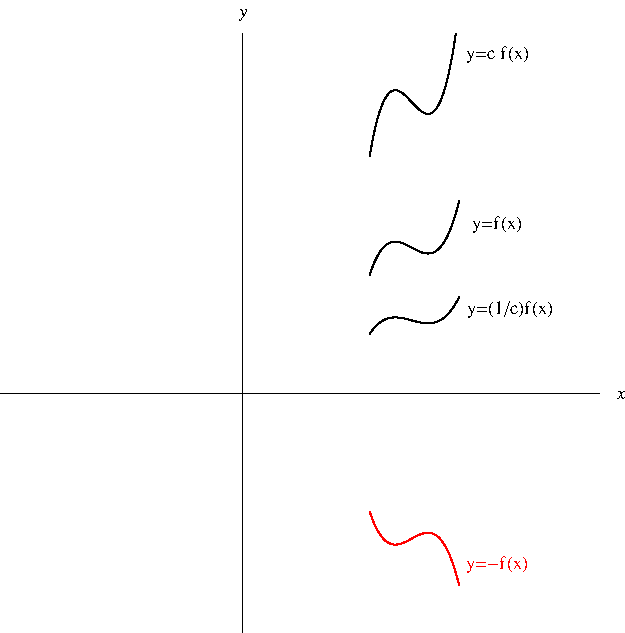
\includegraphics[height=5cm]{precalculus/pictures/01-03-magd.pdf}%
}%
\only<6>{%
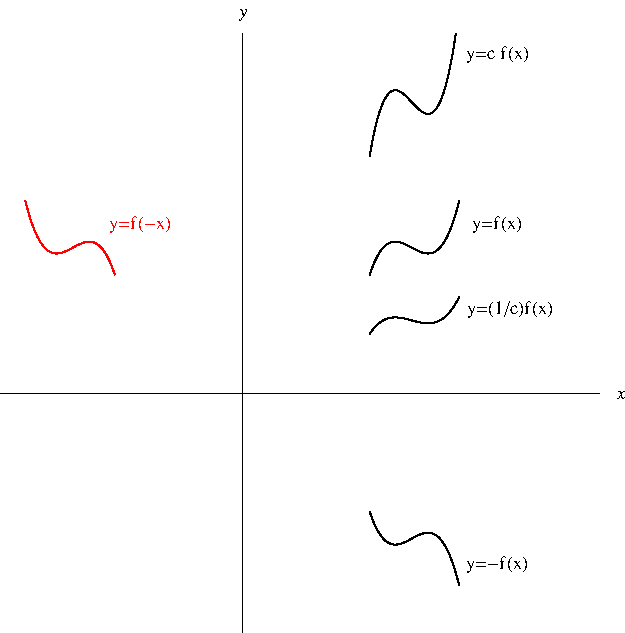
\includegraphics[height=5cm]{precalculus/pictures/01-03-mage.pdf}%
}%a
\column{.5\textwidth}
What happens if we multiply or divide by a constant $c > 1$ in the equation of a function $f$?  What happens if we multiply $f$ by $-1$?  What happens if we multiply $x$ by $-1$ before applying $f$?
\end{columns}

\uncover<2->{
\begin{tabular}{|l|l|}
\hline
\alert<handout:0| 3>{$cf(x)$} &%
\uncover<3->{\alert<handout:0| 3>{Stretch the graph of $f(x)$ vertically by a factor of $c$.}} \\%
\alert<handout:0| 4>{$(1/c)f(x)$} &%
\uncover<4->{\alert<handout:0| 4>{Compress the graph of $f(x)$ vertically by a factor of $c$.}} \\%
\alert<handout:0| 5>{$-f(x)$} &%
\uncover<5->{\alert<handout:0| 5>{Reflect the graph of $f(x)$ in the $x$-axis.}} \\%
\alert<handout:0| 6>{$f(-x)$} &%
\uncover<6->{\alert<handout:0| 6>{Reflect the graph of $f(x)$ in the $y$-axis.}}\\%
\hline
\end{tabular}
}
\end{frame}
% end module transformations-magnifications
